%------------------------------------------------------------ COMMANDS
\newcommand{\sheight}{0.5}
\newcommand{\slength}{10}


%----------------------------------------------------------------------

\begin{figure}
\centering
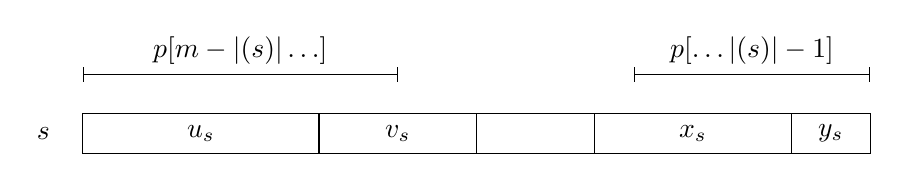
\begin{tikzpicture}%[scale=0.9, every node/.style={scale=0.8}]

%Non terminal A
\node (ha) at (0,0) {};
\node at (-0.5,0.5*\sheight) {$s$};
\draw (ha) rectangle ++ (\slength,\sheight);
\draw (ha) rectangle ++ (3,\sheight) node[midway] {$u_s$};
\draw (3,0) rectangle ++ (2,\sheight) node[midway] {$v_s$};

\draw (6.5,0) rectangle ++ (2.5,\sheight) node[midway] {$x_s$};
\draw (9,0) rectangle ++ (1,\sheight) node[midway] {$y_s$};

\draw [|-|] (0,1) -- (4,1) node [midway, above] {$p[m - |\prefix(s)| \dots]$};
\draw [|-|] (7,1) -- (10,1) node [midway, above] {$p[\dots |\suffix(s)|-1]$};
\end{tikzpicture}
\caption{A \boundaryinfo{$p$} for a string $s$ that is not a substring of $p$.}
\label{fig:pboundary}
\end{figure}